\section{Exemples avec alterqcm.sty et tkz-fct}\label{prof}%
Dans ce chapitre, les exemples sont encore des sujets de Baccalauréat ES utilisant  le module \tkzname{alterqcm.sty} mais aussi les modules dérivés de tikz, \tkzname{tkz-fct.sty} et bien évidemment \tkzname{tkz-tab.sty}.
Vous trouverez des exemples accompagnant cette documentation avec un \textcolor{red}{|préambule minimum|}.
\vfill
\example{Baccalauréat Centres Étrangers ES 2006 }\label{bac1}

\medskip
\begin{alterqcm}[lq=70mm,pre=true]

\AQmessage{ Soit $f$ une fonction définie et dérivable sur l'intervalle $]-5~;~+\infty[$ dont le tableau de variations est donné ci-dessous :
\begin{center}
\begin{tikzpicture}
\tkzTabInit[espcl=1.75]{$x$/1,$f(x)$/3}
 {$-5$,$-1$,$0$,$2$,$+\infty$}
\tkzTabVar{-/$-\infty$ /,%
           +/$-3$/,%
           -/$-5$/,%
           +/4   /,%
           -/{4,5}/}
\end{tikzpicture}
\end{center}
 On désigne par $\mathcal{C}$  la courbe représentative de $f$.}


\AQquestion{Sur l'intervalle $]-5~;~+\infty[$, l'équation $f(x) = -2$ admet }
{{une seule solution},
{deux solutions},
{quatre solutions}
}
\AQquestion{Sur l'intervalle $]-5~;~+\infty[$ la courbe $\mathcal{C}$ admet : }
{%
{\begin{minipage}{6cm}\small une seule asymptote  la droite d'équation $x = -5$%
\end{minipage}},
{\begin{minipage}{6cm}\small exactement deux asymptotes, les droites d'équations $x = -4,5$ et $y = -5$%
\end{minipage}},
{\begin{minipage}{6cm}\small exactement deux asymptotes, les droites d'équations $y = -4,5$ et $x =  -5$%
\end{minipage}}%
}
\AQquestion{On sait que $f'(2) = 0$. L'équation de la tangente à $\mathcal{C}$ au point d'abscisse $2$ est : }
{{$y  = 4$},
{$y = 4(x -2)$},
{$y = 4(x -2)$}
}
\AQquestion{On sait que l'équation de la tangente à $\mathcal{C}$ au point de coordonnées (1 ; 2) est $y = 3x - 1$. On a :}
{{$f(2) = 1$},
{$f'(1) = -1$},
{$f'(1) = 3$}
}
\AQquestion{Sur l'intervalle $]2~;~+\infty[$, la fonction $g$ définie par $g(x) =\text{e}^{-f(x)}$ }
{{est croissante},
{est décroissante},
{n'est pas monotone.}
}
\AQquestion{On pose $h(x) = \ln \left[f(x) + 5\right]$. Alors la fonction $h$ : }
{{$\mathbb{R}$},
{$]0~;~+\infty[$},
{$[0~;~+\infty[$}
}
\end{alterqcm}


\vfill
\example{Baccalauréat ES Antilles juin 2004 }\label{bac2}

\medskip

\begin{alterqcm}[lq=110mm,pre=true]

\AQmessage{ La figure 1. donne la représentation graphique d'une fonction $f$ définie sur $\mathbf{R}^+$ et la figure 2 celle d'une primitive de $f$ sur $\mathbf{R}^+$.
\begin{center}
 \begin{tikzpicture}[xscale=2.25,yscale=1]
    \tkzInit[xmin=-2,xmax=3,ymin=-1,ymax=6]
    \tkzX
    \tkzY
    \tkzFct[label=false,samples=100](-1..2.2){x+exp(x-1)}
    \tkzPoint[noname,coord](1,2){pt1}
    \tkzPoint[noname,coord,label,xlabel={},%
              ylabel=$\text{e}+2$,posylabel=10pt]%
             (2,2+e){pt2}
    \tkzRep
 \end{tikzpicture}
\end{center}
\begin{center}
  \begin{tikzpicture}[xscale=2.25,yscale=1]
    \tkzInit[xmin=-2,xmax=3,ymin=-1,ymax=6]
    \tkzX
    \tkzY
    \tkzFct(-2..2.2){x*x/2+exp(x-1)}
    \tkzPoint[noname,coord,label,xlabel={},ylabel=$3/2$](1,1.5){pt1}
    \tkzPoint[noname,coord,label,xlabel={},%
             ylabel=$\text{e}+2$,posylabel=10pt]%
            (2,2+e){pt2}
   \tkzRep
  \end{tikzpicture}
\end{center}
}

\AQquestion{Quelle est l'aire, en unités d'aire, de la partie du plan limitée par la représentation graphique de la fonction $f$, l'axe des abscisses et les
droites d'équation $x = 1$ et $x = 2$ ? }
{{$\text{e} + \cfrac{3}{4}$},
{$\text{e} + \cfrac{1}{2}$},
{$1$}
}

\end{alterqcm}

\medskip
\hfill Tournez la page s.v.p.


\begin{alterqcm}[lq=70mm,pre=false,numbreak=1]
\AQmessage{La fonction $k$ définie et strictement positive sur $\mathbf{R}^+$ est connue par son tableau de variations.
\begin{center}
\begin{tikzpicture}
     \tkzTabInit[lgt=1,espcl=2]{$x$/0.5,$k(x)$/1.5}
     {$0$,$1$,$3$,$+\infty$}
     \tkzTabVar{-/            /,%
                +/            /,%
                -/            /,%
                +/ $+\infty$  /}%
     \end{tikzpicture}
\end{center}%
}

\AQquestion{Pami les tableaux suivants, quel est le tableau de variations de la fonction $g$ définie sur
$\mathbf{R}^+$ par \[g(x) = \cfrac{1}{k(x)}\ ? \]}
{{Tableau A},
{Tableau B},
{Tableau C}
}

\AQmessage{%
\begin{center}
Tableau A\\
\begin{tikzpicture}
     \tkzTabInit[lgt=1,espcl=2]{$x$/0.5,$g(x)$/1.5}
     {$0$,$1$,$3$,$+\infty$}
     \tkzTabVar{-/            /,%
                +/            /,%
                -/            /,%
                +/ $+\infty$  /}%
     \end{tikzpicture}
\end{center}
\begin{center}
Tableau B\\
\begin{tikzpicture}\activoff
     \tkzTabInit[lgt=1,espcl=2]{$x$/0.5,$g(x)$/1.5}
     {$0$,$1$,$3$,$+\infty$}
     \tkzTabVar{+/            /,%
                -/            /,%
                +/            /,%
                -/ $-\infty$  /}%
     \end{tikzpicture}
\end{center}
\begin{center}
Tableau C\\
\begin{tikzpicture}\activoff
     \tkzTabInit[lgt=1,espcl=2]{$x$/0.5,$g(x)$/1.5}
     {$0$,$1$,$3$,$+\infty$}
     \tkzTabVar{-/            /,%
                +/            /,%
                -/            /,%
                +/ $0$        /}%
     \end{tikzpicture}
\end{center}
}

\AQquestion{Soit $h$ la fonction définie sur $\mathbf{R}$ par $h(x) = \text{e}^x - x + 1$.
On note $\mathcal{C}$ la courbe représentative de $h$ dans un repère
orthonormal  $O;\vec{\imath};\vec{\jmath}$.}
{{%
\begin{minipage}{5cm}\small
  La droite d'équation $y = 1$ est
  asymptote à $\mathcal{C}$%
\end{minipage}
},
{\begin{minipage}{5cm}\small
 La droite d'équation $x = 0$ est
asymptote à $\mathcal{C}$
\end{minipage}},
{\begin{minipage}{5cm}\small
 La droite d'équation $y = -x + 1$ est
asymptote à $\mathcal{C}$
\end{minipage}}
}
\AQquestion[pq=5mm]{%
En économie, le coût marginal est le coût occasionné par la
production d'une unité supplémentaire, et on considère que le coût
marginal est assimilé à la dérivée du coût total.\\
Dans une entreprise, une étude a montré que le coût marginal
$C_{m}(q)$ exprimé en millliers d'euro en fonction du nombre $q$
d'articles fabriqués est donné par la relation :
\[C_{m}(q) = 3q^2 - 10q + \cfrac{2}{q} + 20.\]
}
{%
{$C_{r}(q) = q^3 - 5q^2 + 2\ln q + 20q + 9984$},
{$C_{r}(q) = q^3 - 5q^2 + 2\ln q + 20q - 6$},
{$C_{r}(q) = 6q - 10 - \cfrac{2}{q^2}$}
}

\end{alterqcm}
\vfill

\endinput